\documentclass{article}

\usepackage[final]{neurips_2026}
\makeatletter
\renewcommand{\@noticestring}{} % suppress the "38th Conference on..." footer the template adds under [final]
\makeatother

\usepackage[utf8]{inputenc}
\usepackage[T1]{fontenc}
\usepackage{hyperref}
\usepackage{url}
\usepackage{booktabs}
\usepackage{amsfonts}
\usepackage{amsmath}
\usepackage{nicefrac}
\usepackage{microtype}
\usepackage{xcolor}
\usepackage{graphicx}
\usepackage{placeins}
\renewcommand{\arraystretch}{1.0}
\setlength{\tabcolsep}{4pt}
\setlength{\textfloatsep}{4pt plus 1pt minus 1pt}
\setlength{\floatsep}{4pt plus 1pt minus 1pt}
\setlength{\intextsep}{4pt plus 1pt minus 1pt}
\setlength{\abovecaptionskip}{3pt}
\setlength{\belowcaptionskip}{1pt}
\renewcommand{\topfraction}{0.9}
\renewcommand{\bottomfraction}{0.9}
\renewcommand{\textfraction}{0.05}
\renewcommand{\floatpagefraction}{0.7}
\setcounter{topnumber}{4}
\setcounter{bottomnumber}{4}
\setcounter{totalnumber}{8}


\title{CS 6304 PA1 \\ \large (``Beyond IID: Inductive Biases, Unsupervised Domain Adaptation, Domain Generalization, and Open-Set Recognition'')}

\author{%
  Laeeba Hafeez Malik \\
  CS 6304 - ATML\\
  \texttt{28100027@lums.edu.pk}
}

\begin{document}

\maketitle

\begin{abstract}
Models that match training and test distributions closely (the standard IID, closed-set
assumption) can still fail once that assumption is relaxed. This report studies four such
failures, all run with one fixed seed (6304): (1) which visual cues a ResNet-50, a ViT-B/16, and
CLIP ViT-B/32 rely on under color, cue-conflict, translation, and patch-shuffle interventions on
Oxford-IIIT Pets; (2) whether unlabeled target access helps a ResNet-18 adapt from three PACS
source domains (Photo, Art Painting, Cartoon) to Sketch via DAN, DANN, and CDAN; (3) whether the
same backbone can generalize to Sketch \emph{without} ever seeing it, using ERM, source-only MMD
alignment (DAN-DG), and Sharpness-Aware Minimization; and (4) whether a CIFAR-10 classifier can
tell when a CIFAR-100 image belongs to none of its ten classes, comparing four post-hoc novelty
scores (MSP, MLS, Energy, Mahalanobis) and three trained models (Vanilla, GCSC, PROSER). Four
angles, one conclusion: architecture alone does not decide which cues a model uses or how it fails
under shift. Alignment that lowers a domain-separability proxy does not automatically improve
recognition, and can wipe out class information instead. Local flatness and target-free source
invariance do not reliably predict generalization to an unseen domain. And closed-set accuracy is
only loosely coupled to a model's ability to reject genuinely novel inputs. Each claim is backed by
controlled comparisons, training-curve diagnostics, and concrete failure cases, not aggregate
numbers alone.

\medskip
\noindent Code and machine-readable results: \url{https://github.com/laeebahafeez/ATML-PA1}
\end{abstract}

% ============================================================================
\section{Introduction}

Ordinary supervised learning assumes training and test data share a distribution, and that every
test input belongs to a known class. Both assumptions break in deployment: a model trained on
studio photos meets a hand-drawn sketch, and a ten-class classifier meets an eleventh class it has
never seen. This report treats those breakdowns as four experiments unified by one question: what
should a robust representation preserve, what should it become invariant to, and when should it
reject an input rather than force a prediction?

Task 1 asks the preservation question at the level of visual cues. Under interventions that remove
color, swap shape and texture, translate the object, or scramble spatial layout, which cues does a
CNN, a ViT, and a vision-language model actually use, and does that evidence stay visible in their
representations even when predictions do not change? Tasks 2 and 3 ask the invariance question at
the level of domains. Given the same three PACS sources and the same unseen Sketch target, does
suppressing domain identity in the representation, with unlabeled target access in Task 2 or
without it in Task 3, improve recognition, or does it throw away class-discriminative information
along with domain identity? Task 4 asks the rejection question: can a classifier restricted to ten
known classes tell an ordinary mistake apart from an input that never belonged to any of them, and
does that ability track ordinary accuracy or pull apart from it? Section 3 works through each
task's evidence around its research questions; Section 4 returns to the unifying question using
evidence gathered across all four.

% ============================================================================
\section{Experimental Setup}

Across all four tasks we fix a single seed (6304) for every stochastic step, including splits,
initialization, shuffling, augmentation, and random selection, so every reported number traces to
a saved configuration or result file.

\textbf{Task 1.} We evaluate on Oxford-IIIT Pets (37 classes; stratified 20\% validation split;
class-balanced 500-image test subset) rather than the coarser STL-10, since its fine-grained,
breed-level labels should make color and texture reliance easier to see in clean accuracy and the
size of intervention-induced drops. Three frozen backbones are compared: ResNet-50
\cite{he2016resnet} (ImageNet1K-V2 weights), ViT-B/16 \cite{dosovitskiy2021vit} (ImageNet1K-V1),
and CLIP ViT-B/32 \cite{radford2021clip} (OpenAI-pretrained), each with one linear head trained on
top of frozen features (AdamW, lr $10^{-3}$, weight decay $10^{-4}$, up to 50 epochs with early
stopping after 5 epochs without validation-accuracy improvement). CLIP is also evaluated zero-shot
(``a photo of a \{class\}.''). Grayscale is the required color intervention; on top of it we add a
fixed $90^\circ$ hue rotation, on the hypothesis that breed identity is partly color-coded, so a
plausible-but-wrong hue should hurt more than removing color entirely (confirmed in 3.1). For
translation ($0/8/16/32$px, four directions) and patch-shuffle ($4\times4$ grid) we report accuracy
alongside prediction consistency, $\frac{1}{N}\sum_i\mathbf{1}[\hat y(x_i){=}\hat y(T(x_i))]$, the
fraction of predictions unchanged by an intervention. Cue conflicts use full-strength ($\alpha=1$)
AdaIN style transfer \cite{huang2017adain} across five class pairs in both directions; maximal
strength should give the least ambiguous conflicts at the cost of lower coverage, and 240 of 247
attempts passed a rejection rule fixed before any model saw them. We report shape bias,
$N_{\mathrm{shape}}/(N_{\mathrm{shape}}{+}N_{\mathrm{texture}}){\times}100$, alongside coverage,
$(N_{\mathrm{shape}}{+}N_{\mathrm{texture}})/N_{\mathrm{total}}{\times}100$, since shape bias alone
hides predictions that fell into neither intended class. Representations are visualized with t-SNE
(perplexity 30) rather than UMAP, since its emphasis on local neighbor structure should best show
whether transformed examples stay near their clean counterparts; this is quantified as
representation stability, $I_T=\frac{1}{N}\sum_i\cos(f(x_i),f(T(x_i)))$, the average cosine
similarity between each image's clean and transformed feature vector.

\textbf{Tasks 2 and 3.} Both tasks share the PACS \cite{li2017pacs} protocol: Photo, Art Painting,
and Cartoon as sources, Sketch as the held-out target, using an ImageNet1K-V1-pretrained ResNet-18
backbone with BatchNorm statistics frozen for every method, so later domain-separability comparisons
stay fair. Images are resized to 256px and randomly cropped to $224{\times}224$ with horizontal
flipping for training (center-cropped for evaluation); every method uses AdamW (lr $10^{-4}$, weight
decay $10^{-4}$) for up to 30 epochs, with early stopping after 5 epochs without improvement on
source-validation macro-F1. Each training batch draws 8 examples from each of the 3 source domains
(24 total). DAN, DANN, and CDAN additionally draw 24 unlabeled target examples, giving equal
source/target batch sizes. Task 2 compares Source-only ERM against DAN \cite{long2015dan} (a
non-adversarial MMD penalty pulling source and target features together, main
$\lambda_{\mathrm{mmd}}{=}1$), DANN \cite{ganin2016dann} (an adversarial domain discriminator
trained via gradient reversal), and CDAN \cite{long2018cdan} (the same discriminator conditioned on
the predicted class); all four clip gradients to a global norm of 1.0 per step (immaterial for
Source-only/DAN, binding only once DANN/CDAN's gradients spike), applied uniformly to keep the
optimizer fixed across methods.
Task 3 reuses the Task 2 Source-only checkpoint as its ERM baseline, since it
never saw Sketch to begin with, and compares DAN-DG (the identical MMD mechanism, main
$\lambda_{\mathrm{dg}}{=}1$, applied only across the three sources) against SAM
\cite{foret2021sam} (main $\rho{=}0.05$, same optimizer as ERM, no domain-alignment term). We track
domain separability throughout (a simple classifier's held-out accuracy at telling domains apart
from frozen features; chance is 1/2 in Task 2, 1/3 in Task 3), and in Task 3 also a local sharpness
proxy (loss increase after one small adversarial parameter step).

\textbf{Task 4.} All ten CIFAR-10 classes are known, and unknowns come only from fixed CIFAR-100
classes: a near group (bus, pickup\_truck, motorcycle, tractor, wolf, fox, leopard, camel) and a far
group (bottle, bowl, chair, clock, keyboard, mushroom, sunflower, wardrobe), 800 images each, never
used for training, selection, or calibration. A CIFAR-appropriate ResNet-18 is trained from scratch
(random init, not ImageNet-pretrained, with its stem adapted for $32{\times}32$ inputs) for two
closed-set models, Vanilla and GCSC, using SGD (lr 0.1, momentum 0.9, weight decay
$5{\times}10^{-4}$, cosine schedule, 100 epochs) with random-crop and horizontal-flip augmentation.
GCSC's only change is inserting RandAugment after crop/flip, which lets us test whether a stronger
closed-set classifier is incidentally a better open-set one. For both models we report closed-set
accuracy (CSA, ordinary top-1 accuracy on the known classes) alongside near/far AUROC, the
threshold-independent area under the ROC curve for separating known from unknown. On Vanilla's
frozen logits and features we compute four post-hoc scores: MSP \cite{hendrycks2017msp}
($1{-}\max_k p_k$), MLS \cite{vaze2022mls} ($-\max_k z_k$), Energy \cite{liu2020energy}
($-\log\sum_k e^{z_k}$), and Mahalanobis distance \cite{lee2018mahalanobis} to the nearest class
mean. We then fine-tune the selected Vanilla checkpoint into PROSER \cite{zhou2021proser}, adding
five dummy classifiers trained with a classifier-placeholder loss and a manifold-mixup
\cite{verma2019manifoldmixup} data-placeholder loss built only from pairs of known CIFAR-10
examples, so no CIFAR-100 leakage occurs. Rejection
thresholds are calibrated as the 95th percentile of each score on CIFAR-10 validation data; we
report both this rate and the threshold-independent AUROC.

% ============================================================================
\section{Results}

% ---------------------------------------------------------------------------
\subsection{Task 1: Inductive Biases of ResNet, ViT, and CLIP}

\begin{table}[h]
  \centering
  \caption{Clean / grayscale / additional-color (hue rotation) / patch-shuffle top-1 accuracy. Source: \texttt{step1\_clean\_baseline.csv}, \texttt{step2\_color\_bias.csv}, \texttt{step5\_patch\_shuffle.csv}.}
  \label{tab:task1-main}
  \small
  \resizebox{0.92\textwidth}{!}{%
  \begin{tabular}{lcccc}
    \toprule
    Model & Clean acc. & Grayscale acc. & Hue-rotation acc. & Patch-shuffle acc. \\
    \midrule
    ResNet-50 (head)     & 0.908 & 0.856 & 0.806 & 0.784 \\
    ViT-B/16 (head)      & 0.918 & 0.860 & 0.844 & 0.852 \\
    CLIP ViT-B/32 (head) & 0.788 & 0.690 & 0.620 & 0.504 \\
    CLIP ViT-B/32 (zero-shot) & 0.756 & 0.690 & 0.628 & 0.532 \\
    \bottomrule
  \end{tabular}%
  }
\end{table}

\begin{table}[h]
  \centering
  \caption{Shape/texture/other decisions (of 240 cue-conflict examples), shape bias, coverage. Source: \texttt{step3\_shape\_bias.csv}.}
  \label{tab:task1-shapebias}
  \small
  \resizebox{0.98\textwidth}{!}{%
  \begin{tabular}{lccccc}
    \toprule
    Model & Shape dec. & Texture dec. & Other dec. & Shape bias (\%) & Coverage (\%) \\
    \midrule
    ResNet-50 (head)     & 22 & 27 & 191 & 44.9 & 20.4 \\
    ViT-B/16 (head)      & 2  & 1  & 237 & 66.7 & 1.25 \\
    CLIP ViT-B/32 (head) & 4  & 8  & 228 & 33.3 & 5.00 \\
    CLIP ViT-B/32 (zero-shot) & 12 & 21 & 207 & 36.4 & 13.75 \\
    \bottomrule
  \end{tabular}%
  }
\end{table}

\emph{RQ1 (color/cue-conflict).} Every model loses more accuracy from hue rotation than from
grayscale (Table~\ref{tab:task1-main}), even though rotation is not geometrically worse; it merely
replaces color with a different, consistent color. That pattern supports color being diagnostic for
breed identity rather than merely decorative. Cue-conflict coverage is low everywhere
(1.25--20.4\%), so most stylized images are classified as neither the content nor the style breed.
Among decisive predictions every model leans texture or style (ResNet-50: 44.9\% shape bias, i.e.\
55.1\% texture, matching the CNN texture bias reported by Geirhos et al.\
\cite{geirhos2019texturebias}; both CLIP variants sit at 33--36\%). ViT-B/16's 66.7\% figure comes
from only 3 decisions out of 240 and should not be read as ``ViT is shape-biased.'' Its coverage
collapse is the more informative fact here, discussed under RQ3.

\begin{table}[h]
  \centering
  \caption{Selected cue-conflict outcomes across the four models. Source: \texttt{cue\_conflict\_predictions.csv}.}
  \label{tab:task1-cueconflict-examples}
  \small
  \resizebox{\textwidth}{!}{%
  \begin{tabular}{llllll}
    \toprule
    Content / style & ResNet-50 & ViT-B/16 & CLIP (head) & CLIP (zero-shot) & Outcome \\
    \midrule
    Sphynx / Russian Blue   & Sphynx (shape) & Persian (other)    & Sphynx (shape)           & Sphynx (shape) & 3/4 agree: shape \\
    Bombay / Min.\ Pinscher & Bombay (shape) & Birman (other)     & Brit.\ Shorthair (other) & Bombay (shape) & split: 2 shape, 2 other \\
    Russian Blue / Sphynx   & Bombay (other) & Abyssinian (other) & Brit.\ Shorthair (other) & Birman (other) & 4/4 other, all different \\
    Beagle / Staffs.\ Bull Terrier & Sphynx (other) & Bengal (other) & Sphynx (other) & Sphynx (other) & 3/4 agree ``other'', cross-species \\
    Yorkshire / Scottish Terrier   & Bombay (other) & Persian (other) & Brit.\ Shorthair (other) & Bombay (other) & 4/4 other, all cat breeds \\
    \bottomrule
  \end{tabular}%
  }
\end{table}

\textbf{Cue-conflict agreement across models.} No image gets a unanimous verdict. The strongest
cross-model agreement on a decisive answer is 3-of-4, and that happens on only 4 of 240 images (1
shape, row 1; 3 texture). Agreement instead concentrates on failure: at least 3 models say
``other'' on 227 of 240 images (94.6\%), and all four do so, naming four different breeds as row 3
shows, on 160 of them (66.7\%). Row 2's split is not architecture-clean: ResNet-50 and CLIP
zero-shot agree on the correct shape (Bombay), while ViT-B/16 and CLIP's linear probe land on
unrelated breeds instead. So most ``other'' predictions look like genuine failures to resolve
either identity, not muted votes for the unseen cue. Rows 4 and 5 show why this happens, not merely
that it does: both content and style classes there are \emph{dog} breeds, yet three or four of the
four models place the blended image in a \emph{cat} breed instead, never proposing any dog at all
(Section 4 discusses the mechanism). That is the clearest evidence that most ``other'' verdicts
reflect the intervention producing ambiguous or misleading evidence, rather than the models being
generically cautious.

\emph{RQ2 (translation/patch-shuffle).} In Figure~\ref{fig:task1-translation}, accuracy stays
nearly flat for ResNet-50 and ViT-B/16 out to 32px, while CLIP sits roughly 10 points below its own
clean baseline at every displacement including 0, a calibration gap rather than a translation
effect, since it does not widen with distance. Consistency tells a different story. ResNet-50 and
ViT-B/16 stay at 0.95--0.99, but CLIP drops to 0.86--0.90: roughly 1 in 8 CLIP predictions flip
under a shift that barely moves its aggregate accuracy, plausibly because CLIP's $32{\times}32$
patches make a 32px shift exactly one patch width, the worst possible grid misalignment.
Patch-shuffling hurts CLIP far more (head: $-$28.4 pts, consistency 0.51) than ResNet-50
($-$12.4) or, notably, ViT-B/16 ($-$6.6). The supervised ViT is, in fact, \emph{least} disrupted
by destroying global layout, which cuts against the intuition that positional tokens should make it
the most layout-sensitive model. Pretraining objective looks like the better explanation than
architecture here: CLIP's contrastive training rewards holistic composition, so scrambling patches
destroys exactly the evidence it relies on.

\begin{figure}[h]
  \centering
  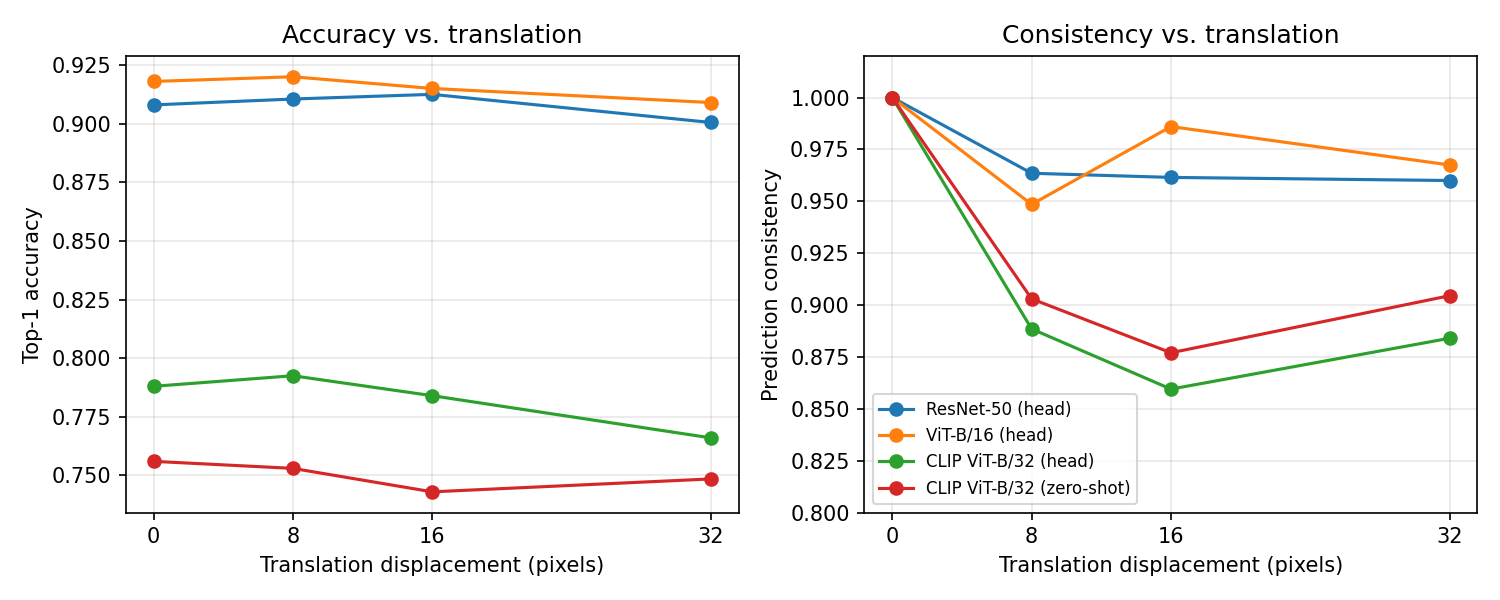
\includegraphics[width=0.68\textwidth]{figures/task1_translation_curve.png}
  \caption{Accuracy (left) and prediction consistency (right) vs.\ translation displacement. Source: \texttt{step4\_translation\_*.csv}.}
  \label{fig:task1-translation}
\end{figure}

\emph{RQ3 (predictions vs.\ representations).} Table~\ref{tab:task1-stability} and
Figure~\ref{fig:task1-tsne} give two clear mismatches. Under patch-shuffle, CLIP has the worst
prediction consistency (0.51) yet the \emph{highest} feature-cosine stability of the three (0.777).
Its embedding barely rotates even as its argmax flips on half of all images, because cosine
stability only checks overall direction, not which side of the decision boundary a feature lands
on. Under cue-conflict, CLIP's stability (0.591) is an order of magnitude above ResNet-50's (0.069)
or ViT-B/16's ($-$0.009, indistinguishable from orthogonal). Figure~\ref{fig:task1-tsne} shows why:
for ViT-B/16, every transformed image, regardless of class, lands in one shared region disjoint
from the clean clusters, so style transfer erases class identity entirely, matching its near-zero
coverage. CLIP's transformed images also separate from its clean clusters but keep enough per-image
structure that paired cosine similarity stays high, plausibly reflecting its more stylistically
diverse pretraining data. CLIP's zero-shot classifier is also more robust than its own trained head
on every intervention (Table~\ref{tab:task1-main}) and reaches higher cue-conflict coverage
(13.75\% vs.\ 5.00\%), which suggests the head, trained on clean images only, overfits a narrower
slice of the embedding space than the zero-shot rule uses.

\begin{table}[h]
  \centering
  \caption{Cosine representation stability $I_T$ (1.0 = identical direction). Source: \texttt{step6\_representation\_stability.csv}.}
  \label{tab:task1-stability}
  \small
  \begin{tabular}{lcccc}
    \toprule
    Model & Grayscale & Patch-shuffle & Translation (32px) & Cue-conflict \\
    \midrule
    ResNet-50     & 0.855 & 0.703 & 0.950 & 0.069 \\
    ViT-B/16      & 0.794 & 0.653 & 0.965 & $-$0.009 \\
    CLIP ViT-B/32 & 0.908 & 0.777 & 0.970 & 0.591 \\
    \bottomrule
  \end{tabular}
\end{table}

\begin{figure}[h]
  \centering
  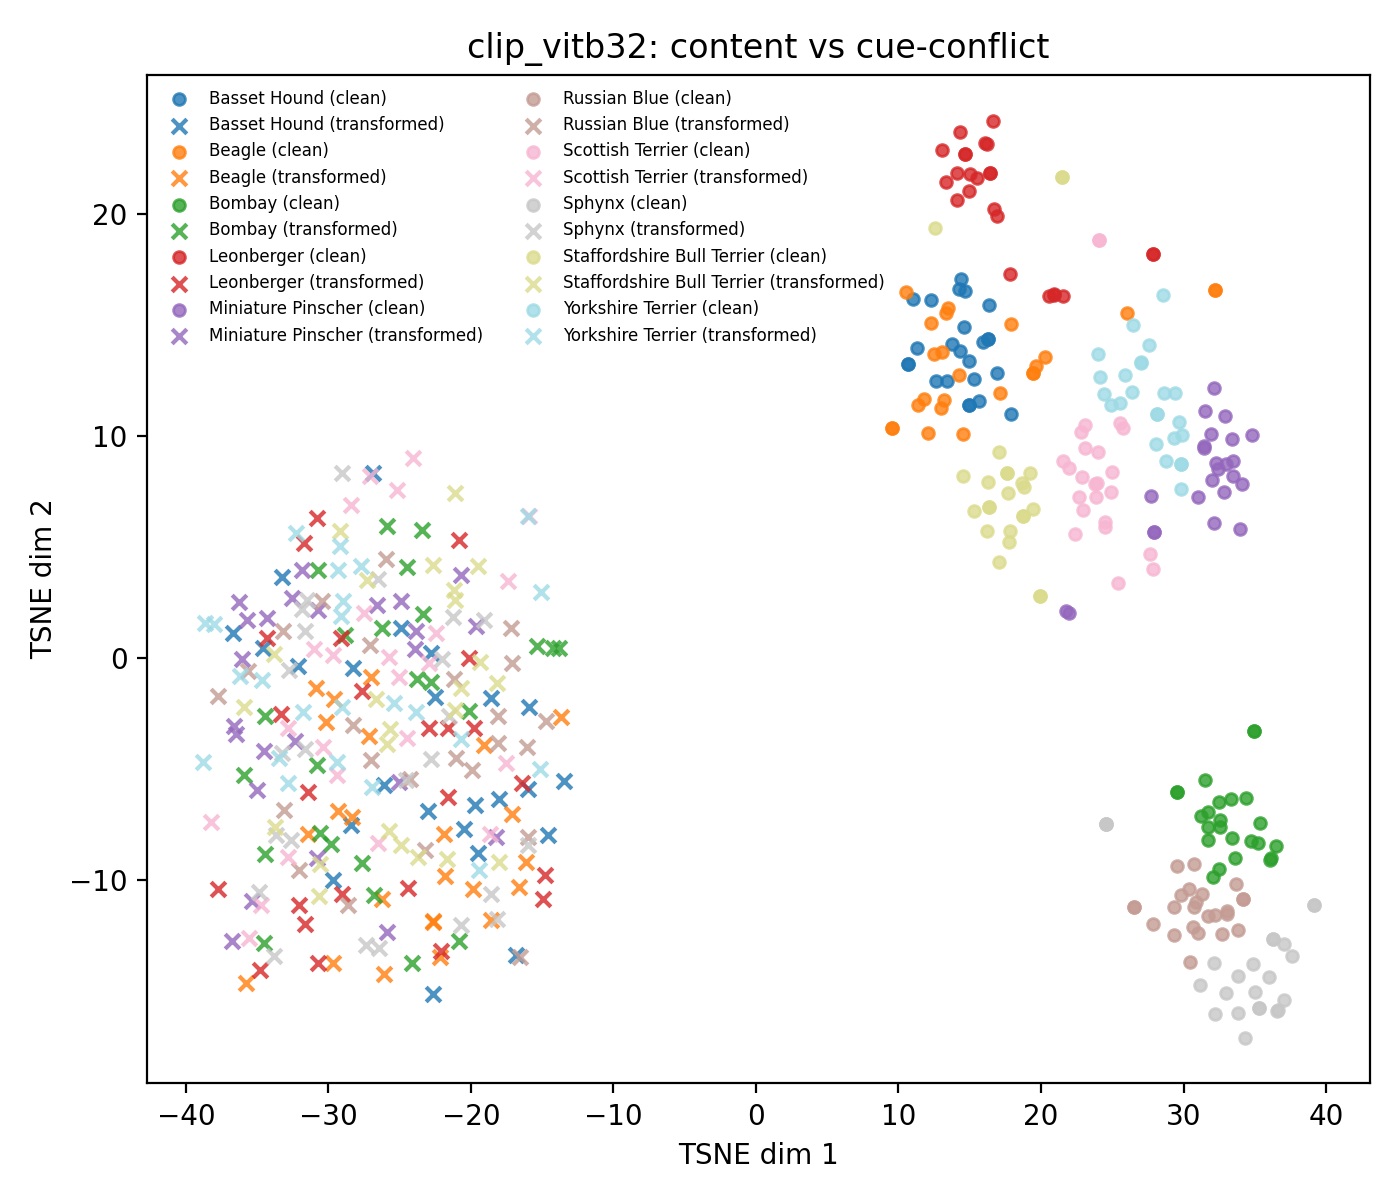
\includegraphics[width=0.49\textwidth]{figures/clip_vitb32_cue_conflict_tsne.png}
  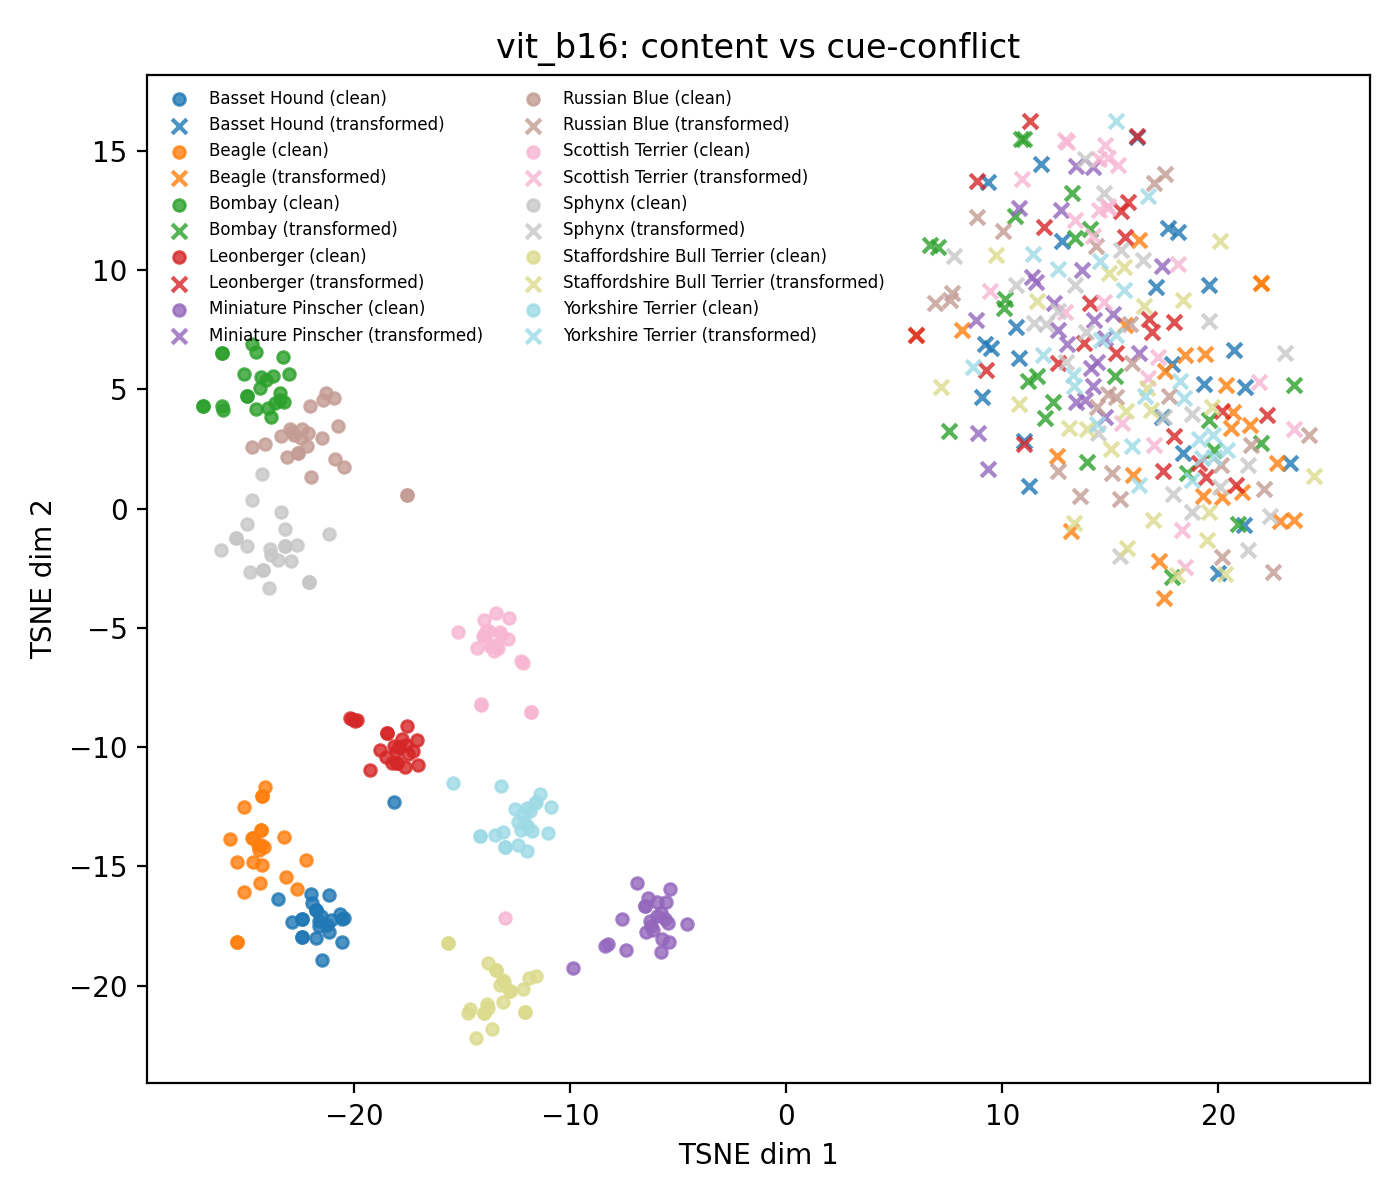
\includegraphics[width=0.49\textwidth]{figures/vit_b16_cue_conflict_tsne.png}
  \caption{t-SNE of clean vs.\ cue-conflict features, CLIP ViT-B/32 (left) and ViT-B/16 (right). Circles = clean, crosses = transformed, color = ground-truth class.}
  \label{fig:task1-tsne}
\end{figure}

\emph{RQ4 (architecture vs.\ data/supervision).} CLIP and ViT-B/16 share a patch-transformer
architecture yet respond oppositely to patch-shuffling ($-$28.4 vs.\ $-$6.6 pts), which tracks
pretraining objective rather than architecture. CLIP's much larger cue-conflict stability plausibly
reflects its stylistically diverse pretraining data: ViT-B/16, architecturally closer to CLIP than
ResNet-50 is, shows the opposite pattern, the lowest stability of the three. One artifact worth
separating from representation quality: CLIP's linear head has mean max-softmax confidence of only
0.064 despite 78.8\% accuracy, far below every other model's 0.77--0.90. That gap comes from an
unscaled linear layer on unit-normalized 512-d embeddings producing small logits, unlike CLIP's own
zero-shot rule, which applies a learned $\approx100\times$ logit scale to the same embeddings. It is
a calibration artifact of how the head was fit, not evidence about the CLIP representation itself.

\FloatBarrier
% ---------------------------------------------------------------------------
\subsection{Task 2: Domain Adaptation (PACS, Sketch as target)}

\begin{table}[h]
  \centering
  \caption{Per-source-domain validation performance and mean-source performance. Source: \texttt{task2/results/main\_comparison.csv}.}
  \label{tab:task2-domains}
  \small
  \resizebox{\textwidth}{!}{%
  \begin{tabular}{lcccccccc}
    \toprule
    & \multicolumn{2}{c}{Photo} & \multicolumn{2}{c}{Art} & \multicolumn{2}{c}{Cartoon} & \multicolumn{2}{c}{Mean src.} \\
    \cmidrule(lr){2-3}\cmidrule(lr){4-5}\cmidrule(lr){6-7}\cmidrule(lr){8-9}
    Method & Acc. & F1 & Acc. & F1 & Acc. & F1 & Acc. & F1 \\
    \midrule
    Source-only & 0.9760 & 0.9718 & 0.9220 & 0.9203 & 0.9254 & 0.9304 & 0.9411 & 0.9408 \\
    DAN         & 0.9670 & 0.9600 & 0.9073 & 0.9064 & 0.9296 & 0.9217 & 0.9346 & 0.9294 \\
    DANN        & 0.9189 & 0.9039 & 0.8512 & 0.8476 & 0.8443 & 0.8315 & 0.8715 & 0.8610 \\
    CDAN        & 0.9700 & 0.9649 & 0.9122 & 0.9099 & 0.9318 & 0.9405 & 0.9380 & 0.9384 \\
    \bottomrule
  \end{tabular}%
  }
\end{table}

\begin{table}[h]
  \centering
  \caption{Target (Sketch) performance, change relative to Source-only, and domain separability. Source: \texttt{task2/results/main\_comparison.csv}.}
  \label{tab:task2-main}
  \small
  \begin{tabular}{lccccc}
    \toprule
    Method & Target acc. & Target F1 & $\Delta$ tgt.\ acc. & Domain sep. \\
    \midrule
    Source-only & 0.6976 & 0.6842 & 0.0000  & 0.9918 \\
    DAN         & 0.7653 & 0.7181 & +0.0677 & 0.8228 \\
    DANN        & 0.1117 & 0.0694 & -0.5859 & 0.9986 \\
    CDAN        & 0.1138 & 0.1312 & -0.5839 & 0.9973 \\
    \bottomrule
  \end{tabular}
\end{table}

\emph{RQ1 (source-to-target gap).} Source-only ERM loses 24.4 points moving to Sketch (0.9411
$\to$ 0.6976). \texttt{Person} is the largest single failure, at 15.0\% Sketch accuracy, with
\texttt{giraffe} a distant second at 42.1\%; the remaining five classes all reach at least 71.2\%.
That is consistent with photographic and cartoon people (and, to a lesser extent, giraffes) looking
least like their sketched counterparts, while rigid objects such as \texttt{house} and
\texttt{guitar} already transfer well with no adaptation at all.

\emph{RQ2 (separability vs.\ recognition).} Table~\ref{tab:task2-domains} shows source performance
is consistent across Photo, Art, and Cartoon for every method, so no single domain is quietly
propping up the mean, and the aggregate comparison in Table~\ref{tab:task2-main} is not hiding
domain-specific behavior. The four methods split sharply. DAN lowers separability from
near-ceiling (0.992) to 0.823 and gains 6.8 points on target: separability and recognition move
together as intended. That gain concentrates unevenly. DAN's largest per-class improvements are
\texttt{person} (0.15$\to$0.99, +0.84) and \texttt{giraffe} (0.42$\to$0.68, +0.26), exactly the two
classes Source-only struggled with most, while \texttt{dog} is the one class DAN makes worse
(0.71$\to$0.57, $-$0.14). This is not a generic accuracy trade-off. DAN's Sketch \texttt{dog}
errors concentrate almost entirely on \texttt{horse} (122 of its misclassified dogs) and
\texttt{person} (102), precisely the two classes whose own regions the alignment pulled hardest
into agreement with Sketch. That points to the shared feature space it builds not being uniformly
better, but reshaping decision boundaries around whichever classes needed the most correction, at
some cost to a class like \texttt{dog} that sits geometrically between them. DANN and CDAN instead
\emph{collapse}: target accuracy falls 58--59 points to near-random while separability stays at
0.997--0.999, essentially unchanged. The adversarial objective did not even achieve domain
confusion, yet it destroyed almost all class structure anyway. Figure~\ref{fig:task2-curves} shows
why: DANN's domain loss sits flat near zero for four epochs, then explodes past 20{,}000 at the
checkpoint epoch, while CDAN's domain and classification losses oscillate together and never
converge. Confusions confirm the mechanism: 67 (DANN) and 75 (CDAN) of \texttt{house}'s
source-validation examples are predicted \texttt{person}, and together with \texttt{person}'s own
jump to 100\% this shows both models degenerating into predicting \texttt{person} almost
everywhere.

\emph{RQ3 (conditional vs.\ marginal alignment).} CDAN's class-conditioning provides no rescue: its
target accuracy (0.1138) is indistinguishable from DANN's (0.1117), with the same collapse. That
makes sense once you consider \emph{why} conditioning is supposed to help. CDAN conditions its
discriminator on the classifier's own predicted class distribution, so the extra signal is only as
good as those predictions are. Figure~\ref{fig:task2-curves} shows CDAN's classification and domain
losses oscillating together rather than one stabilizing the other: once training destabilizes, the
predicted-class information CDAN conditions on becomes unreliable itself, leaving conditioning
nothing trustworthy to condition on. The decisive factor here is adversarial versus statistical
alignment, not marginal versus conditional. DAN's non-adversarial MMD converges smoothly and helps;
both gradient-reversal variants destabilize training and hurt regardless of conditioning.

\begin{figure}[h]
  \centering
  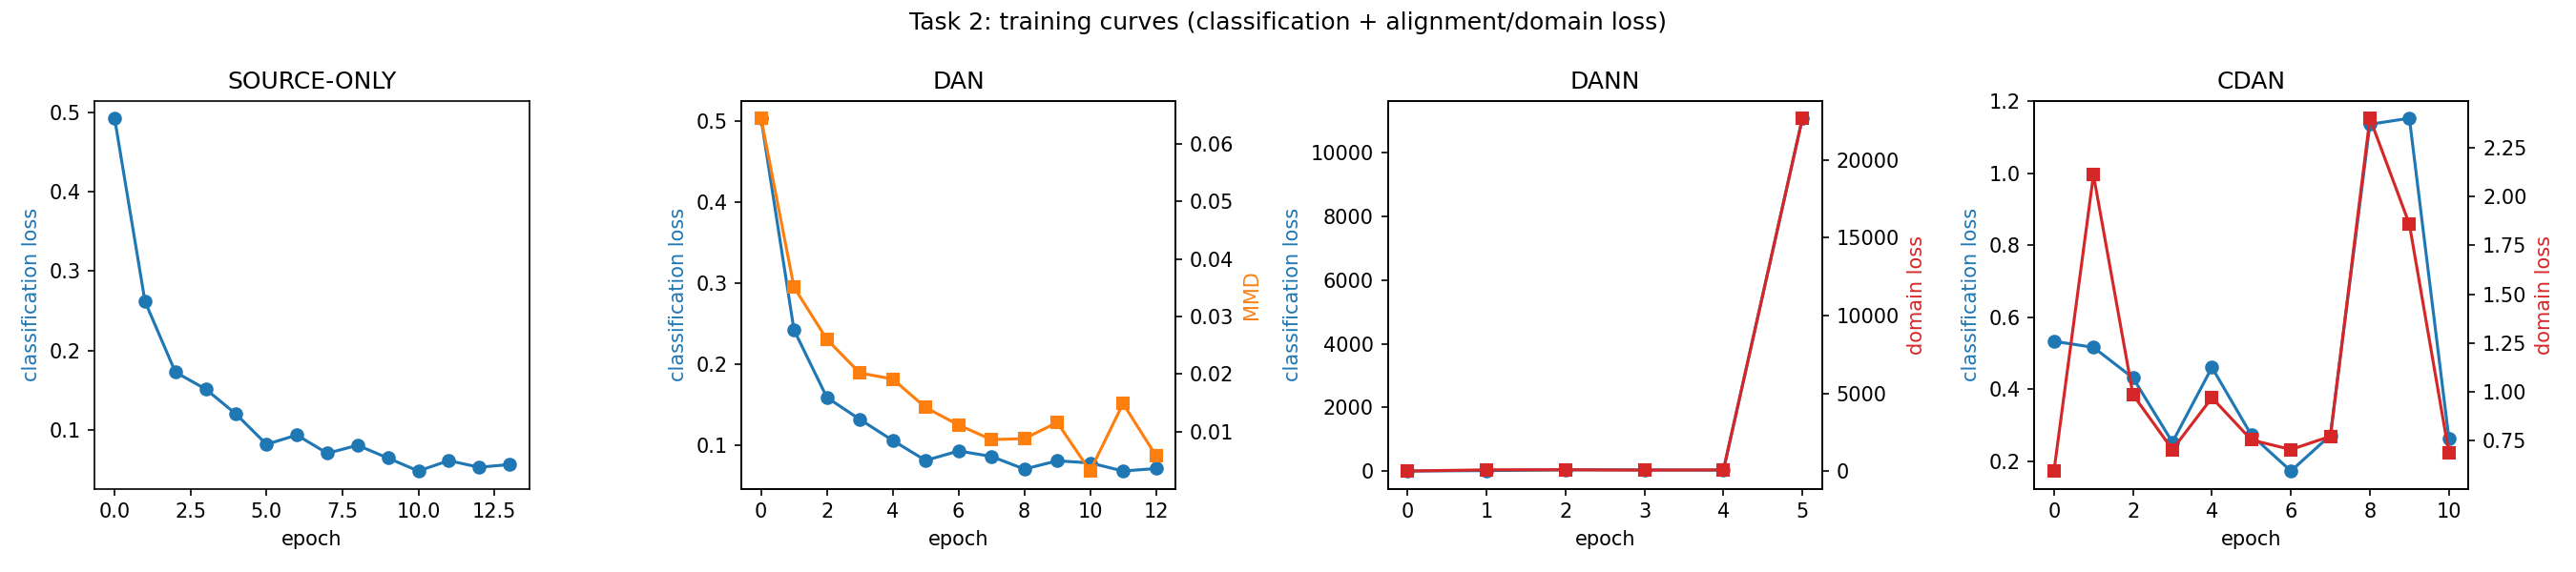
\includegraphics[width=0.85\textwidth]{figures/task2_training_curves_combined.png}
  \caption{Classification and alignment/domain-loss curves, Source-only/DAN/DANN/CDAN. Source: \texttt{task2/results/train\_history\_*.json}.}
  \label{fig:task2-curves}
\end{figure}

\emph{RQ4 (controlled alignment strength).} Table~\ref{tab:task2-controlled-vals} and
Figure~\ref{fig:task2-lambda} sweep $\lambda_{\mathrm{mmd}}\in\{0.1,1,10\}$. Target accuracy peaks
at the main setting ($\lambda=1$, 0.765); weak alignment under-corrects (0.716), and strong
alignment over-corrects, simultaneously hurting source accuracy (0.943$\to$0.895) \emph{and}
raising separability back up (0.880$\to$0.901) instead of continuing to fall. That is optimization
instability, not a smooth trade-off. The non-monotonic separability curve in
Figure~\ref{fig:task2-lambda} (right) makes this visible directly: separability first drops as
$\lambda$ grows from 0.1 to 1, then rises again at $\lambda=10$, tracing a V-shape rather than the
steadily-decreasing curve a simple ``more alignment pressure, less separability'' story would
predict. At $\lambda=10$ the MMD term dominates the classification loss enough to destabilize
training itself, rather than continuing to smoothly align the two domains. Source accuracy and
separability both flag $\lambda=10$ as unsafe without ever consulting target labels: it is the only
setting where source accuracy drops sharply \emph{and} separability climbs back up instead of
continuing to fall, the same two-sided warning sign RQ2 used to diagnose DANN and CDAN's collapse.
Comparing only $\lambda=0.1$ and $\lambda=1$ on source-side evidence alone would still favor
$\lambda=1$, since it reaches the lower, more-reduced separability (0.823 vs.\ 0.881) that the
alignment objective is designed to produce, while its source-accuracy cost relative to
$\lambda=0.1$ is small (0.935 vs.\ 0.943) and shows none of $\lambda=10$'s instability. That
source-only-justified choice happens to land on the actual best target setting, which suggests the
source-side diagnostics are not useless. They simply cannot tell a merely safe setting apart from the
optimal one the way target evaluation can.

\begin{table}[h]
\centering
\caption{Controlled DAN study: effect of $\lambda_{\mathrm{mmd}}$. Source: \texttt{controlled\_study\_dan\_lambda\_mmd.csv}.}
\label{tab:task2-controlled-vals}
\begin{tabular}{lccc}
\toprule
$\lambda_{\mathrm{mmd}}$ & Mean src.\ acc. & Target acc. & Domain sep. \\
\midrule
0.1 & 0.9432 & 0.7160 & 0.8805 \\
1.0 (main) & 0.9346 & 0.7653 & 0.8228 \\
10.0 & 0.8946 & 0.6383 & 0.8901 \\
\bottomrule
\end{tabular}
\end{table}

\begin{figure}[h]
  \centering
  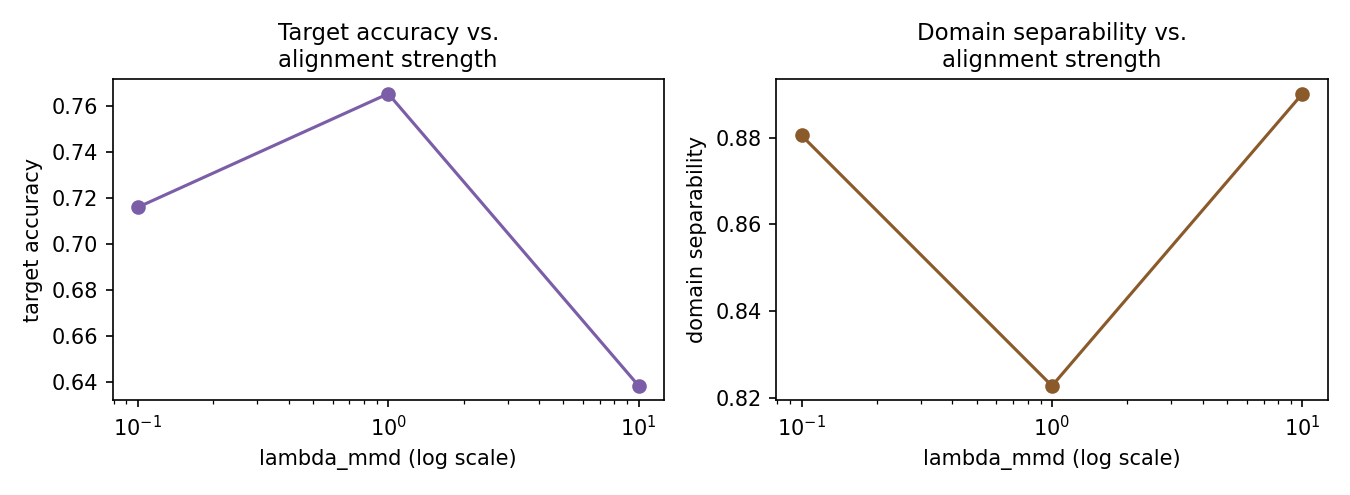
\includegraphics[width=0.76\textwidth]{figures/controlled_study_dan_lambda_mmd.png}
  \caption{Controlled $\lambda_{\mathrm{mmd}}$ study: target accuracy (left) and domain separability (right) vs.\ alignment strength. Source: \texttt{controlled\_study\_dan\_lambda\_mmd.csv}.}
  \label{fig:task2-lambda}
\end{figure}

\FloatBarrier
% ---------------------------------------------------------------------------
\subsection{Task 3: Domain Generalization (PACS, Sketch held out)}

\begin{table}[h]
  \centering
  \caption{Per-source-domain validation performance, mean- and worst-source. Source: \texttt{task3/results/main\_comparison.csv}.}
  \label{tab:task3-domains}
  \small
  \resizebox{\textwidth}{!}{%
  \begin{tabular}{lcccccccccc}
    \toprule
    & \multicolumn{2}{c}{Photo} & \multicolumn{2}{c}{Art} & \multicolumn{2}{c}{Cartoon} & \multicolumn{2}{c}{Mean src.} & \multicolumn{2}{c}{Worst src.} \\
    \cmidrule(lr){2-3}\cmidrule(lr){4-5}\cmidrule(lr){6-7}\cmidrule(lr){8-9}\cmidrule(lr){10-11}
    Method & Acc. & F1 & Acc. & F1 & Acc. & F1 & Acc. & F1 & Acc. & F1 \\
    \midrule
    ERM     & 0.9760 & 0.9718 & 0.9220 & 0.9203 & 0.9254 & 0.9304 & 0.9411 & 0.9408 & 0.9220 & 0.9203 \\
    DAN-DG  & 0.9700 & 0.9650 & 0.9098 & 0.9134 & 0.9147 & 0.9231 & 0.9315 & 0.9338 & 0.9098 & 0.9134 \\
    SAM     & 0.9760 & 0.9730 & 0.9439 & 0.9418 & 0.9382 & 0.9447 & 0.9527 & 0.9532 & 0.9382 & 0.9418 \\
    \bottomrule
  \end{tabular}%
  }
\end{table}

\begin{table}[h]
  \centering
  \caption{Sketch performance, change relative to ERM, source-domain separability, and sharpness. Source: \texttt{task3/results/main\_comparison.csv}.}
  \label{tab:task3-main}
  \small
  \resizebox{\textwidth}{!}{%
  \begin{tabular}{lccccc}
    \toprule
    Method & Sketch acc. & Sketch F1 & $\Delta$ vs.\ ERM & Dom.\ sep. & Sharpness \\
    \midrule
    ERM     & 0.6976 & 0.6842 & 0.0000  & 0.8600 & 0.2788 \\
    DAN-DG  & 0.6808 & 0.6262 & -0.0168 & 0.7700 & 0.2797 \\
    SAM     & 0.6455 & 0.6719 & -0.0522 & 0.8633 & 0.1209 \\
    \bottomrule
  \end{tabular}%
  }
\end{table}

\emph{RQ1 (do source metrics predict Sketch?).} Poorly, and in the wrong direction. SAM has the
best mean- and worst-source accuracy of the three, yet the \emph{worst} Sketch accuracy ($-$5.2
pts); DAN-DG has the weakest source numbers but a smaller Sketch drop ($-$1.7).
Table~\ref{tab:task3-domains} confirms this is not one weak domain distorting the mean: all three
sources move together for every method. Per-class evidence shows why the aggregate misleads.
DAN-DG's \texttt{house} collapses on Sketch from 93.75\% to 27.5\% (confused mostly as
\texttt{giraffe} and \texttt{elephant}), the same \texttt{house} that, per Task 2's RQ1, already
transferred well with \emph{no} adaptation at all, so this failure is specific to DAN-DG's
cross-source alignment rather than an inherently hard class. SAM's \texttt{dog} drops 22.5 points,
with 276 of its Sketch confusions landing on \texttt{elephant} alone: large, class-specific
failures that are invisible in any aggregate source number.

\emph{RQ2 (does DAN-DG's invariance help?).} DAN-DG meets its own target: source-domain
separability falls from 0.86 to 0.77. But that invariance does not transfer, since Sketch accuracy
ends up slightly \emph{worse} than ERM's. The \texttt{house} failure above suggests the alignment
removed information useful for separating rigid-object silhouettes, not merely domain identity.

\emph{RQ3 (does SAM's flatness predict Sketch performance?).} SAM's sharpness proxy (0.121) is
under half of ERM's (0.279) and DAN-DG's (0.280, unchanged from ERM as expected). But ranked by
flatness, SAM $\ll$ ERM $\approx$ DAN-DG, while ranked by Sketch accuracy, ERM $>$ DAN-DG $>$ SAM:
the exact reverse order. Local stability, by this proxy, does not predict Sketch generalization
here, and the proxy's own definition suggests why not. It perturbs parameters by a small step and
measures the loss increase \emph{on held-out source data}, so it only certifies that the loss
surface is flat in directions relevant to the three observed sources. Sketch is a large,
qualitatively different shift (line drawings versus photos, paintings, and cartoons), not a small
perturbation along any direction SAM's gradient-ascent step would explore. A solution can therefore
be flat with respect to source perturbations while still sitting in a region that generalizes
poorly along the specific direction separating sources from Sketch. Flatness here is a claim about
the neighborhood SAM actually samples, not about robustness to shift in general.

\begin{figure}[h]
  \centering
  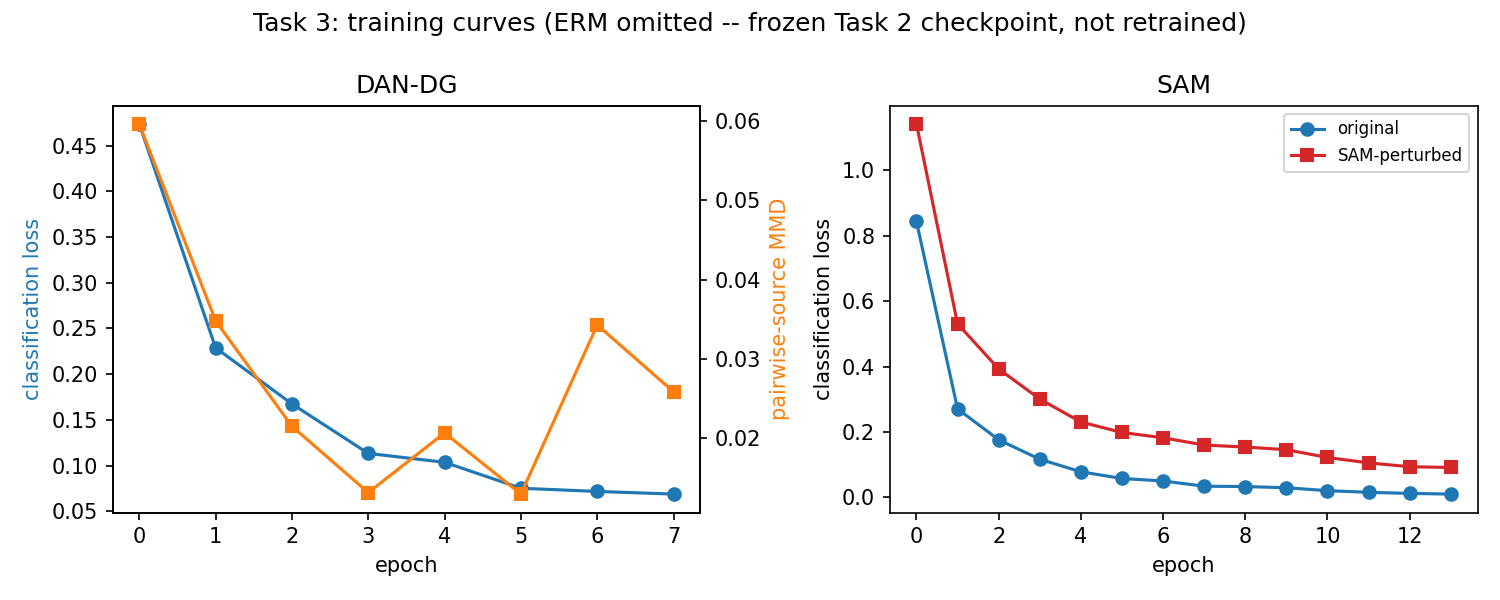
\includegraphics[width=0.72\textwidth]{figures/task3_training_curves_combined.png}
  \caption{Classification loss (MMD penalty for DAN-DG; original vs.\ SAM-perturbed loss for SAM). ERM reuses the Task 2 Source-only checkpoint, so has no curve of its own.}
  \label{fig:task3-curves}
\end{figure}

The controlled study (Table~\ref{tab:task3-controlled-vals} and Figure~\ref{fig:task3-lambda})
sharpens this picture. The \emph{weakest} setting, $\lambda_{\mathrm{dg}}=0.1$, gives the best
Sketch accuracy of any Task 3 run (0.727, beating ERM), while the main setting under-performs ERM
and $\lambda_{\mathrm{dg}}=10$ collapses training outright (source accuracy 0.381, sharpness 1.90).
Separability does not explain the ranking either: $\lambda=0.1$'s 0.797 exceeds $\lambda=1$'s
0.770, yet generalizes better. Useful invariance strength has a narrow range, and either too little
or too much (or outright optimization failure) can dominate the outcome.
Figure~\ref{fig:task3-lambda} (right) shows the sharpness proxy's sudden, order-of-magnitude jump
between $\lambda=1$ and $\lambda=10$ (log scale, 0.28$\to$1.90) lining up exactly with the
source-accuracy collapse (left panel) rather than a gradual trade-off, consistent with
$\lambda=10$ destabilizing optimization outright rather than simply over-aligning.

\begin{table}[h]
\centering
\caption{Controlled DAN-DG study: effect of $\lambda_{\mathrm{dg}}$. Source: \texttt{controlled\_study\_dan\_dg.csv}.}
\label{tab:task3-controlled-vals}
\begin{tabular}{lcccc}
\toprule
$\lambda_{\mathrm{dg}}$ & Mean src.\ acc. & Sketch acc. & Source dom.\ sep. & Sharpness \\
\midrule
0.1 & 0.9508 & 0.7272 & 0.7967 & 0.2403 \\
1.0 (main) & 0.9315 & 0.6808 & 0.7700 & 0.2797 \\
10.0 & 0.3814 & 0.1682 & 0.7000 & 1.8977 \\
\bottomrule
\end{tabular}
\end{table}

\begin{figure}[h]
  \centering
  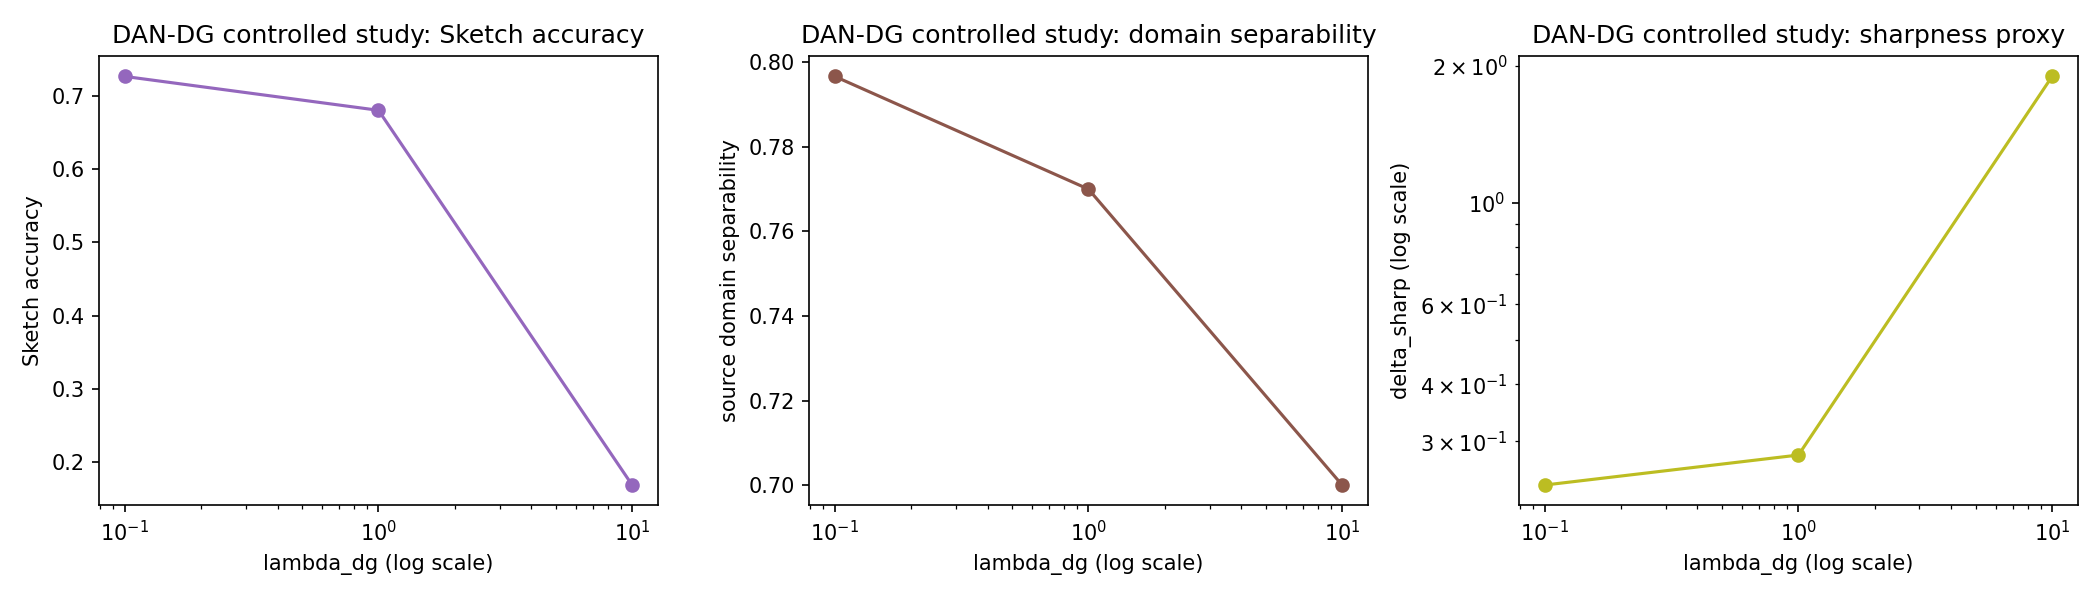
\includegraphics[width=0.78\textwidth]{figures/controlled_study_dan_dg.png}
  \caption{Controlled $\lambda_{\mathrm{dg}}$ study: Sketch accuracy, source-domain separability, and sharpness proxy (log scale) vs.\ alignment strength. Source: \texttt{controlled\_study\_dan\_dg.csv}.}
  \label{fig:task3-lambda}
\end{figure}

\emph{RQ4 (target-aware DAN vs.\ target-free DAN-DG).} Both apply the same MMD mechanism at
$\lambda=1$; the only difference is whether the aligned target is real unlabeled Sketch (DAN) or
only the three sources (DAN-DG). DAN reaches 0.765 Sketch accuracy and DAN-DG reaches 0.681, an
8.5-point gap under otherwise matched settings, and DAN-DG's best controlled configuration (0.727)
still falls short of DAN's main result. Table~\ref{tab:task2-vs-task3-perclass} makes the mechanism
behind that gap concrete at the class level, comparing DAN's Task 2 changes directly with DAN-DG's
Task 3 changes for the same seven Sketch classes.

\begin{table}[h]
  \centering
  \caption{Per-class Sketch accuracy change vs.\ the shared Source-only/ERM baseline: target-aware DAN (Task 2) vs.\ target-free DAN-DG (Task 3). Source: \texttt{task2/results/per\_class\_dan\_vs\_source\_only.csv}, \texttt{task3/results/per\_class\_dan\_dg\_vs\_erm.csv}.}
  \label{tab:task2-vs-task3-perclass}
  \small
  \begin{tabular}{lccc}
    \toprule
    Class & Baseline acc.\ & DAN $\Delta$ (Task 2) & DAN-DG $\Delta$ (Task 3) \\
    \midrule
    person   & 0.150 & +0.838 & +0.363 \\
    giraffe  & 0.421 & +0.260 & +0.270 \\
    horse    & 0.721 & +0.063 & +0.042 \\
    guitar   & 0.924 & +0.058 & -0.132 \\
    elephant & 0.845 & -0.062 & +0.069 \\
    dog      & 0.712 & -0.141 & -0.361 \\
    house    & 0.938 & +0.063 & -0.663 \\
    \bottomrule
  \end{tabular}
\end{table}

Both mechanisms agree closely on \texttt{person} and \texttt{giraffe}, the two classes
Source-only/ERM struggled with most (+0.84/+0.36 and +0.26/+0.27). Both classes are already
somewhat inconsistent in appearance across only Photo, Art, and Cartoon, so pulling those three
domains together, which is all DAN-DG ever does, already builds a more style-general notion of
``person'' or ``giraffe'' that happens to transfer to Sketch, with no need to have ever seen a
Sketch image. The two methods sharply disagree on \texttt{house}: DAN leaves it essentially
untouched (+0.06), while DAN-DG collapses it by 66 points, confused mostly as \texttt{giraffe} and
\texttt{elephant}. \texttt{house} was already one of the best-transferring classes under no
adaptation at all (Task 2's RQ1), so it did not need correcting. DAN can tell this, because it gets
to see (unlabeled) real Sketch houses during training and can implicitly calibrate how much
adjustment each class actually needs. DAN-DG cannot, since it never sees Sketch, so it applies the
same cross-source alignment pressure to \texttt{house} as to every other class, distorting a
representation that did not need to move until it drifts into unrelated classes' regions.
\texttt{dog} shows the same asymmetry more mildly ($-$0.14 vs.\ $-$0.36): both degrade, but DAN-DG
degrades it over twice as much with no target-side signal to limit the damage. Together, this
suggests the main value of unlabeled target access is not raising the ceiling on the hardest
classes, since generic cross-source alignment already does much of that job blind, but knowing
\emph{where alignment should stop}: avoiding damage to classes that were already fine.

This is suggestive, not a clean causal isolation, for three concrete reasons. First, it uses a
single seed (6304) throughout, so we cannot rule out that the specific per-class pattern, rather
than the general direction of the effect, is partly a property of this one run. Second, DAN's
Sketch access is not a single isolated bit flipped on top of an otherwise identical procedure:
every DAN training batch literally contains 24 additional (unlabeled) Sketch examples that DAN-DG's
batches never see, so DAN's advantage bundles together ``having any access to real target
structure'' with ``training on a different, larger effective batch each step,'' and we cannot
cleanly attribute the gap to the former alone. Third, the two methods were not explored with equal
thoroughness. The controlled study (Table~\ref{tab:task3-controlled-vals}) shows DAN-DG is quite
sensitive to $\lambda_{\mathrm{dg}}$, with its weakest setting beating its own main result, but
DAN's $\lambda_{\mathrm{mmd}}$ sweep (Table~\ref{tab:task2-controlled-vals}) uses the same
three-point grid rather than an exhaustive search for its own best configuration. So this compares
each method's \emph{default} recipe, not the best each mechanism could plausibly achieve, and a
wider search on either side could narrow or widen the 8.5-point gap reported here.

\FloatBarrier
% ---------------------------------------------------------------------------
\subsection{Task 4: Open-Set Recognition (CIFAR-10 known / CIFAR-100 unknowns)}

\begin{table}[h]
  \centering
  \caption{MSP / MLS / Energy / Mahalanobis on the frozen vanilla model. Source: \texttt{scores\_comparison\_vanilla.csv}.}
  \label{tab:task4-scores}
  \small
  \resizebox{0.92\textwidth}{!}{%
  \begin{tabular}{lcccccc}
    \toprule
    Score & Near AUROC & Far AUROC & All AUROC & Near rej. & Far rej. & All rej. \\
    \midrule
    MSP         & 0.8235 & 0.8921 & 0.8578 & 0.2950 & 0.4450 & 0.3700 \\
    MLS         & 0.8070 & 0.8862 & 0.8466 & 0.3288 & 0.5163 & 0.4225 \\
    Energy      & 0.8073 & 0.8867 & 0.8470 & 0.3288 & 0.5263 & 0.4275 \\
    Mahalanobis & 0.7984 & 0.9149 & 0.8567 & 0.2825 & 0.5075 & 0.3950 \\
    \bottomrule
  \end{tabular}%
  }
\end{table}

\begin{table}[h]
  \centering
  \caption{Vanilla / GCSC / PROSER: CSA and near/far OSR metrics (MLS common score; PROSER's own placeholder score as an extra row). Source: \texttt{models\_comparison.csv}.}
  \label{tab:task4-models}
  \small
  \begin{tabular}{lcccc}
    \toprule
    Model (score) & CSA & Near AUROC / rej. & Far AUROC / rej. \\
    \midrule
    Vanilla (MLS)              & 0.9474 & 0.807 / 0.329 & 0.886 / 0.516 \\
    GCSC (MLS)                 & 0.9504 & 0.811 / 0.343 & 0.891 / 0.579 \\
    PROSER (MLS)               & 0.9435 & 0.804 / 0.301 & 0.858 / 0.338 \\
    PROSER (placeholder score) & 0.9435 & 0.792 / 0.318 & 0.885 / 0.489 \\
    \bottomrule
  \end{tabular}
\end{table}

\emph{RQ1 (semantic similarity and rejection).} Near AUROC (0.80--0.82) trails far AUROC
(0.89--0.91) for every score, as designed. Among the ten most confidently-accepted failures in each
group (vanilla, MLS), \texttt{bus}$\to$\texttt{truck} recurs most on the near side (6 of 10),
followed by \texttt{pickup\_truck}$\to$\texttt{automobile} (3 of 10) and a single
\texttt{fox}$\to$\texttt{cat}. Two vehicle labels, \texttt{truck} and \texttt{automobile}, absorb 9
of these 10 near failures between them. On the far side no label dominates nearly as much:
\texttt{mushroom}$\to$\texttt{frog} recurs 3 times, \texttt{bottle}$\to$\texttt{cat} and
\texttt{chair}$\to$\texttt{airplane} twice each, and \texttt{bowl} splits between \texttt{cat} and
\texttt{ship} once each, with one \texttt{clock}$\to$\texttt{bird}. Five different known labels
absorb five distinct far classes, each only a handful of times, versus two labels absorbing three
near classes almost entirely. Near failures are semantically coherent (\texttt{bus}/\texttt{truck}
and \texttt{pickup\_truck}/\texttt{automobile} are genuinely similar vehicle shapes;
\texttt{fox}/\texttt{cat} share size and posture), matching why these classes were grouped as
``near'' in the first place and why they collapse onto so few labels. Far failures look more
idiosyncratic and spread thinly across more labels: rarer overall, but more like incidental feature
overlap than category confusion.

\begin{table}[h]
  \centering
  \caption{Selected near/far failures (vanilla, MLS): most confident incorrect acceptances. Source: \texttt{failures\_near.csv}, \texttt{failures\_far.csv}.}
  \label{tab:task4-failures}
  \small
  \begin{tabular}{llccc}
    \toprule
    Type & Unknown class & Predicted class & Score & Threshold \\
    \midrule
    Near & fox           & cat      & -11.593 & -5.764 \\
    Near & bus           & truck    & -11.150 & -5.764 \\
    Near & bus           & truck    & -11.021 & -5.764 \\
    Far  & bowl          & cat      & -12.282 & -5.764 \\
    Far  & bottle        & cat      & -11.697 & -5.764 \\
    Far  & bowl          & ship     & -11.329 & -5.764 \\
    \bottomrule
  \end{tabular}
\end{table}

\emph{RQ2 (what each score captures).} MSP has the highest near AUROC (0.8235); Mahalanobis has the
highest far AUROC (0.9149) and the lowest near AUROC (0.7984), the opposite ranking. MSP's
softmax-bounded margin is most sensitive near a real decision boundary but saturates once a
prediction is already confident, so it cannot distinguish ``fairly sure'' from ``extremely sure.''
MLS keeps the raw, unnormalized top logit instead, so it stays informative in exactly that
saturated regime. Energy aggregates \emph{all} class logits via log-sum-exp rather than only the
top one, which additionally captures diffuse evidence with no single dominant class; that is why
MLS and Energy track each other closely without being identical. Mahalanobis ignores the logits
entirely and uses only feature-space distance, so it is most sensitive to gross shift regardless of
classifier confidence. Logit magnitude proves most informative not by AUROC but at the
actual operating threshold: MLS and Energy give the two highest far-rejection rates of all four
scores (51.6\%, 52.6\%) despite Mahalanobis's better far AUROC, and similarly reject more near
unknowns (32.9\%) than MSP (29.5\%) despite MSP's higher near AUROC. Unbounded logit magnitude
grows the further an input sits from training data, which can separate outliers well at one
specific cutoff even when a bounded or purely geometric score ranks better on average.

\begin{figure}[h]
  \centering
  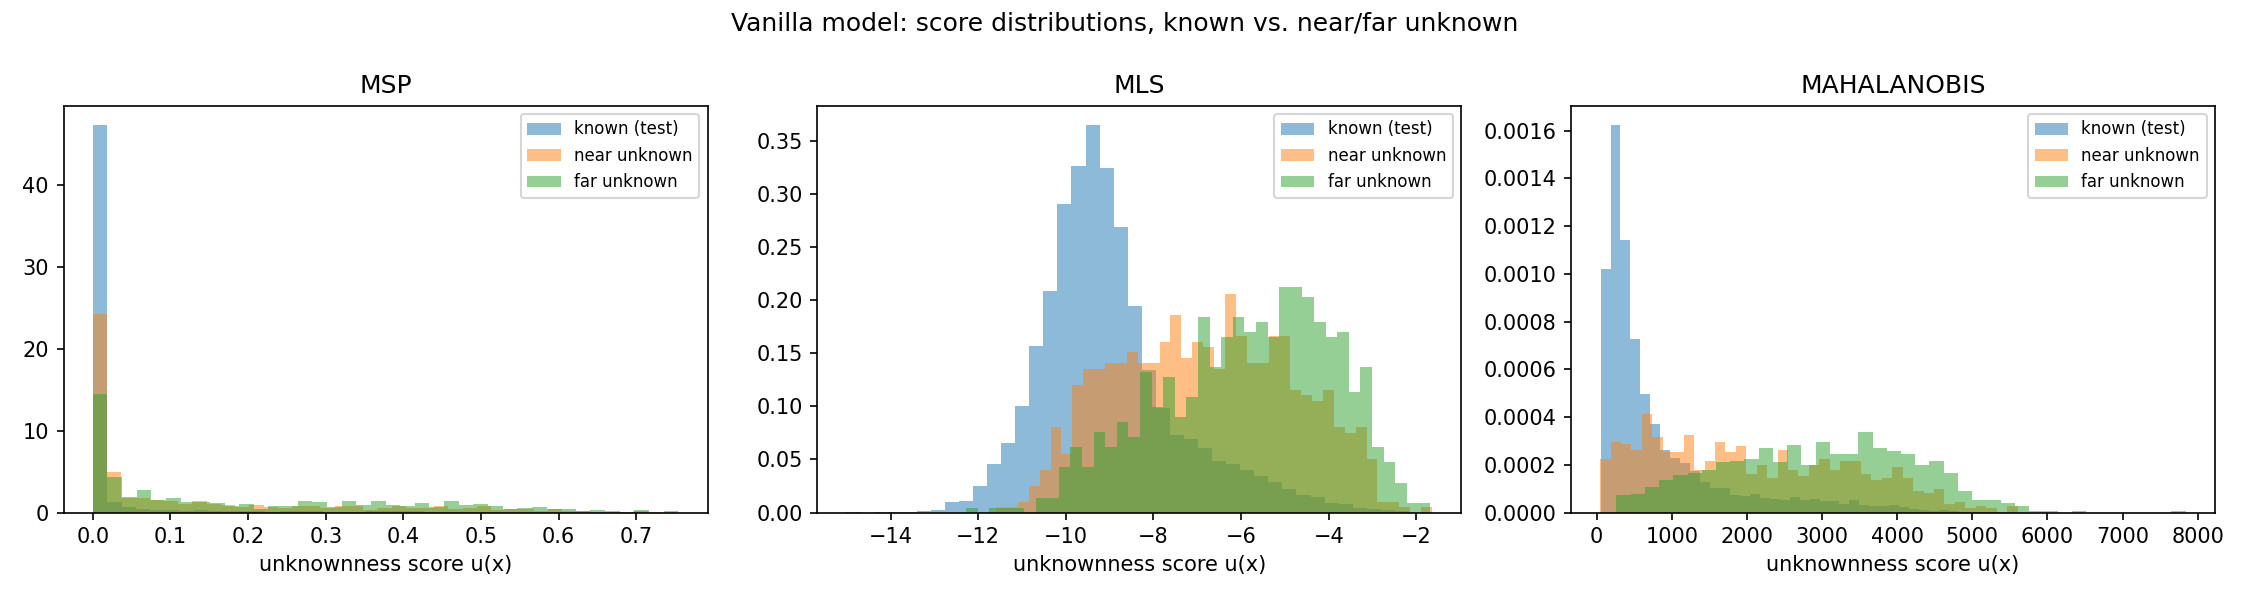
\includegraphics[width=0.82\textwidth]{figures/score_distributions.png}
  \caption{MSP, MLS, and Mahalanobis score distributions, known (test) vs.\ near vs.\ far unknown, frozen vanilla model.}
  \label{fig:task4-scores}
\end{figure}

\emph{RQ3 (does GCSC's augmentation help?).} Both, mildly, and never at a cost. GCSC improves
closed-set accuracy (0.9474$\to$0.9504) and both near and far AUROC (+0.4, +0.5 pts). The larger
effect shows up at the calibrated operating point for far unknowns: rejection jumps
51.6\%$\to$57.9\%, against a small 32.9\%$\to$34.3\% move for near. Stronger closed-set
augmentation builds somewhat more compact known-class regions that incidentally flag grossly
different inputs better, with no open-set objective involved at all. The near/far asymmetry
follows from what ``more compact'' can and cannot fix. A far unknown sits nowhere near any
known-class region to begin with, so shrinking those regions' boundaries inward directly widens the
empty space around it and makes it easier to flag. A near unknown, a wolf for instance, sits close
to a genuinely similar known class (dog) in feature space no matter how tightly that known region
is drawn. Tightening the boundary does not move the wolf itself further from the dog region, so a
near-miss stays a near-miss almost independent of how compact the known classes become.

\emph{RQ4 (does PROSER improve rejection?).} No, in this run, and not only at the far extreme.
PROSER's CSA (0.9435) is below Vanilla and GCSC, and neither of its scores beats Vanilla's AUROC or
rejection on \emph{either} side. With MLS, near AUROC and rejection are both slightly worse than
Vanilla's (0.807$\to$0.804, 0.329$\to$0.301), and far is where the real damage shows up (AUROC
0.886$\to$0.858, rejection 51.6\%$\to$33.8\%). With its own placeholder score, far rejection
(48.9\%) still trails Vanilla, and near AUROC (0.792) trails as well. This is a more complete
failure than the placeholder mechanism's own logic would predict. The classifier- and
data-placeholder losses are specifically meant to tighten the boundaries \emph{between pairs of
known classes}, which should, if anything, help most with near-misses, yet even the near-unknown
numbers did not improve. Its manifold-mixup placeholders interpolate only between pairs of the ten
known classes, a plausible proxy for a near-miss between two known classes in principle, but the
near-unknowns actually tested here (real CIFAR-100 classes like \texttt{fox} or \texttt{wolf}) are
not literal blends of two CIFAR-10 classes, so even that intended sweet spot was not reliably
captured. Interpolation between known classes proves insufficient both for a real,
semantically unrelated far-unknown approaching from outside that space altogether, and, more
surprisingly, for the near-unknowns it was arguably best positioned to help. This reads as a
legitimate negative result rather than a training failure: checkpoint selection followed the same
protocol as Vanilla and GCSC.

\textbf{Positive augmentation vs.\ PROSER.} GCSC (implicit, general augmentation) and PROSER (explicit,
targeted placeholder training) are two different strategies for the same trade-off, directly comparable
against the same Vanilla baseline with the same MLS score. Despite the more targeted design, the
general-purpose strategy wins on every number reported above: GCSC helps closed-set accuracy and all six
AUROC/rejection figures; PROSER helps none of them. Section 4 discusses why: what each method's proxy
for ``unknown'' looks like during training determines what kind of real unknown it generalizes to.

\FloatBarrier
% ============================================================================
\section{Cross-task Discussion}

\textbf{Visual cues and distribution shift.} Task 1 shows color is more than decorative for every
backbone, and CLIP is uniquely hurt by losing global layout; PACS shift (Tasks 2 and 3) changes
color statistics, rendering style, and layout all at once. This is a qualitative parallel, not a
causal claim, since the datasets, architectures, and training regimes all differ. But the
consistent theme is that no cue category is safe to assume irrelevant, and vulnerability tracks
pretraining objective as much as architecture. Two Task 1 results make the ``objective, not
architecture'' half of that claim concrete rather than qualitative. First, CLIP and ViT-B/16 share
a patch-transformer architecture yet respond oppositely to patch-shuffling ($-$28.4 vs.\ $-$6.6
accuracy points). CLIP's contrastive pretraining rewards holistic image-text composition, so
scrambling patches destroys exactly the evidence it relies on, while the supervised ViT is
comparatively undisturbed despite its positional tokens. Second, the cue-conflict examples where
full-strength AdaIN transfer produces images that three or four of four models place in a
\emph{cat} breed despite both source classes being dog breeds
(Table~\ref{tab:task1-cueconflict-examples}, rows 4--5) show that a nuisance-cue intervention can
manufacture inputs that are, in the model's own feature space, genuinely closer to a class neither
source class intended, independent of any single architecture's inductive bias.

\textbf{Invariance vs.\ discriminability.} Across Tasks 2 and 3, a lower separability or sharpness
number is neither necessary nor sufficient for better recognition. DAN is the one case where lower
separability and higher target accuracy move together, with stable training curves. Because MMD is
a smooth statistical distance, it provides a well-behaved gradient throughout training, so the
model can reduce it gradually while classification loss keeps improving alongside it. DANN and CDAN
fail to even reduce separability while collapsing class structure, which the divergent domain-loss
curves diagnose directly: their minimax objective pits the discriminator against the feature
extractor, and once one side starts to dominate (Section 3.2, RQ2 and RQ3), the resulting gradients
stop being informative about domain identity at all and instead simply push features toward whatever
destroys the discriminator's current signal, class structure included. DAN-DG and SAM each hit
their own targeted proxy (lower source separability, lower sharpness) without collapse, yet neither
beats plain ERM on Sketch. SAM, the best source-side performer on every proxy, generalizes worst,
because both proxies are measured only with respect to the three observed sources and have no
mechanism to certify anything about a direction as different as Sketch. These proxies need to be
checked against class-level and target-domain evidence, not trusted on their own.

\textbf{The importance of target domain access.} With unlabeled target access, DAN reaches 0.7653
Sketch accuracy. The identical mechanism restricted to observed sources, DAN-DG, reaches only
0.6808, below the no-adaptation ERM baseline (0.6976). Section 3.3's RQ4 breaks this down per
class: target access matters less for raising the ceiling on the hardest classes (\texttt{person}
and \texttt{giraffe} improve similarly either way) and more for knowing \emph{where alignment
should stop}. DAN-DG, blind to Sketch, keeps ``correcting'' an already-fine \texttt{house} until it
breaks, while DAN does not. That section also details why this falls short of a clean causal
isolation: one seed, a batch-composition confound, and asymmetric hyperparameter search.

\textbf{Recognition vs.\ rejection.} GCSC shows a better closed-set classifier can also be a
modestly safer one: accuracy and both near and far rejection improve together. PROSER breaks that
pattern in both directions. It costs closed-set accuracy \emph{and} fails to improve rejection,
showing an explicitly open-set method can still underperform a plain classifier if its proxy
unknowns (interpolations between known classes) do not resemble the real unknowns it is tested
against. The contrast is informative about \emph{why}, not merely \emph{that}. GCSC's RandAugment
perturbs real known-class images with no explicit notion of ``unknown'' at all, so any rejection
benefit is a side-effect of a generally more compact known-class representation, useful against any
kind of shift. PROSER's manifold-mixup placeholders are explicitly targeted at carving out
low-confidence regions, but only \emph{between} pairs of known classes, which can plausibly help a
near-miss between two known classes but supplies no signal about the far side of the decision
boundary, where most real unknowns, especially far ones, actually sit. A general-purpose
regularizer with no open-set objective transferred to rejection better here than a purpose-built
method whose proxy unknowns did not resemble the real ones it was tested against. Every method's
near-unknown numbers also move less than its far-unknown numbers, echoing Task 1's coverage
warning: aggregate numbers can hide which regime actually changed.

\textbf{Overall synthesis.} The safest generalization here is a negative one: architecture, a
domain-invariance proxy, a flatness proxy, and closed-set accuracy are each informative but
individually unreliable stand-ins for the property they are meant to predict, and each needs
class-level or target-domain checking. What should be preserved is class-discriminative structure,
which DANN and CDAN, and to a lesser extent DAN-DG and PROSER, damaged while pursuing a different,
plausible objective. What should become invariant is only nuisance variation that carries no class
information. DAN's moderate, stable alignment is the one case that struck this balance, while every
method that pushed invariance too hard destroyed discriminative structure along with it. What
should be rejected rather than forced into a label is exactly what Task 4 formalizes, with the
near/far distinction setting how hard that judgment is and which score suits it.

% ============================================================================
\section{Conclusion}

Four experiments framed as one question point to the same answer from different directions. Clean
accuracy, architecture family, and simple invariance or flatness proxies are each informative but
individually unreliable guides outside the IID, closed-set setting they were measured under. Task 1
shows architecture does not cleanly predict cue reliance or spatial sensitivity; pretraining
objective and data matter at least as much. Tasks 2 and 3 show a method can satisfy its own stated
objective without improving, and in the adversarial cases while actively destroying, the
recognition it was meant to serve. Task 4 shows closed-set accuracy and open-set rejection are only
loosely coupled. Section 4 grounds each of these claims in concrete, class-level evidence rather
than aggregate numbers alone. The practical implication is to treat shape bias, domain
separability, sharpness, and closed-set accuracy as diagnostics checked against class-level and
target-distribution evidence, not as targets optimized and trusted in isolation. When a proxy for a
hard-to-measure quantity is unavoidable, ask what kind of failure that proxy is blind to before
trusting it.

\bibliographystyle{plain}
\bibliography{references}

\end{document}
